\documentclass[24 pts]{article}
\usepackage{xeCJK}
\usepackage{amssymb}
\usepackage{amsmath}
\usepackage{amsthm}
\usepackage{graphicx}
\graphicspath{ {images/} }
\setCJKmainfont[BoldFont= Yu Mincho Demibold]{MS Mincho}
\title{整数リング上において置換多項式を使用するターボ符号のためのインタリーバ}
\date{}
\begin{document}
\maketitle

入力:入力重み4エラーイベント(2個の入力重み2エラーイベント。)$\,[0 1 1 0 0 1 1 0\,]$\\
洋装符号;$\frac{1+D^2}{1+D+D^2 }$  8進数 $5/7$\\
置換多項式のインタリーバ:$2x^2+x+3$


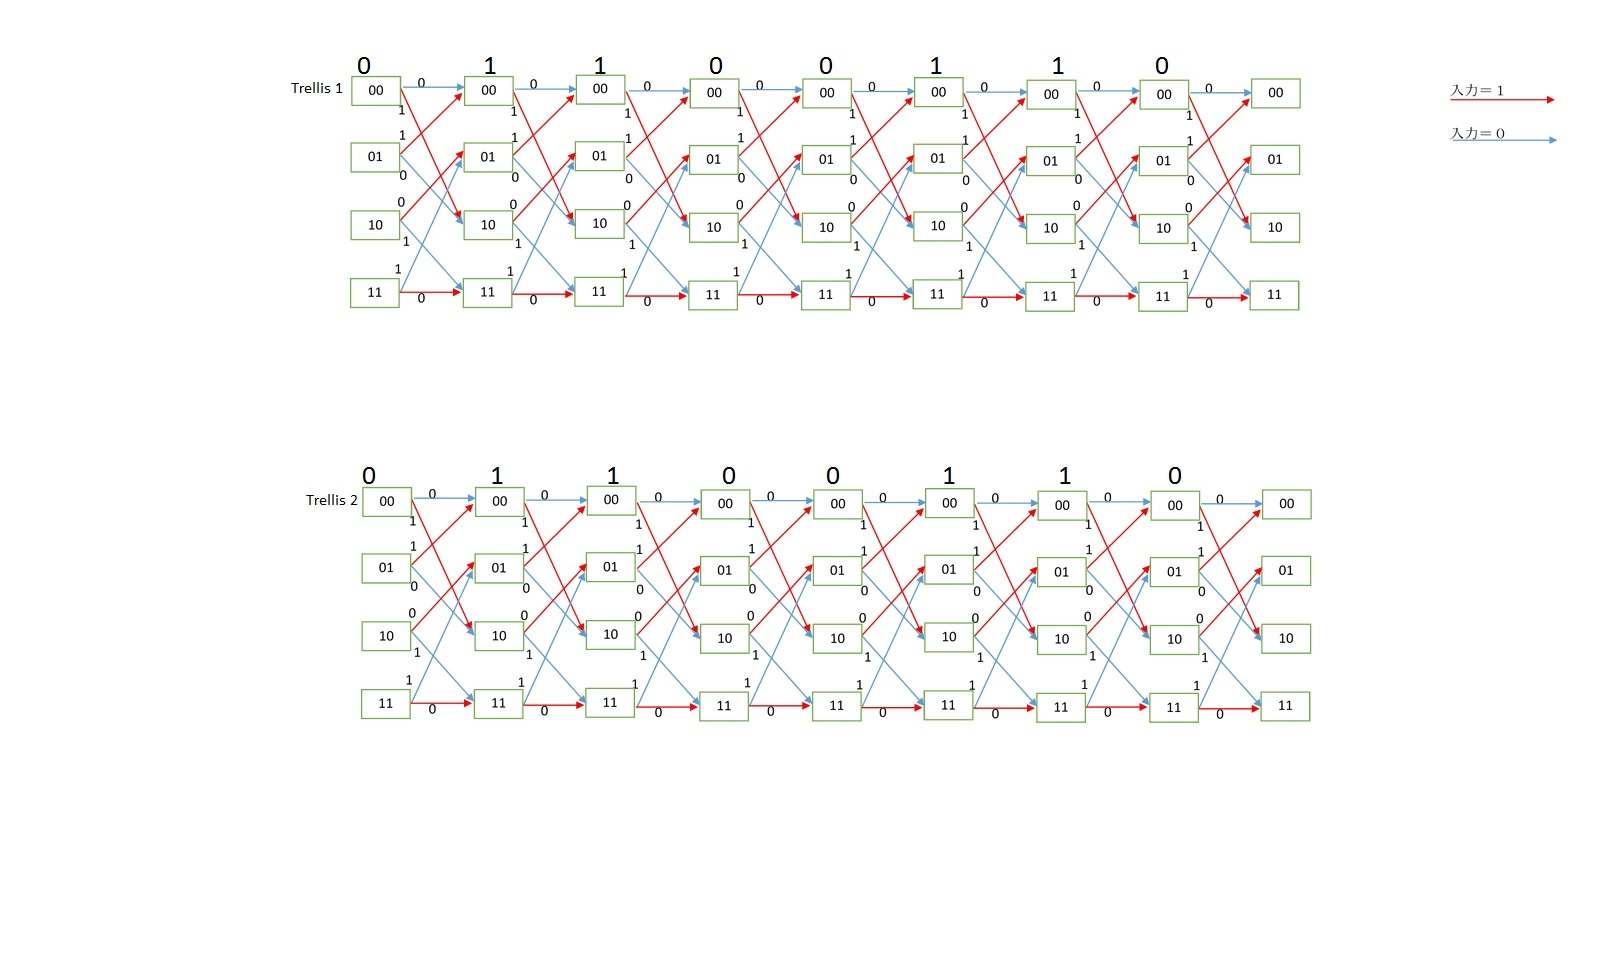
\includegraphics[scale =0.4]{Trellis}\\
\end{document}

